\chapter{\ChapterTitleResults}
\label{sec:wyniki-projektu}

\section{Weryfikacja realizacji wstępnych założeń}

W~pierwszym etapie planowania projektu utworzony został ogólny
plan, który opisywał oddzielne systemy i~elementy
zleconej aplikacji (Rys. \ref{fig:figma_strategicplan}).
Uwzględnia on nie tylko wymagania zdefiniowane w~rozdziale drugim
\nameref{sec:zakres-funkcjonalnosci}, ale także potrzebne do ich
realizacji wymagania techniczne.

\begin{figure}[h!]
    \centering
    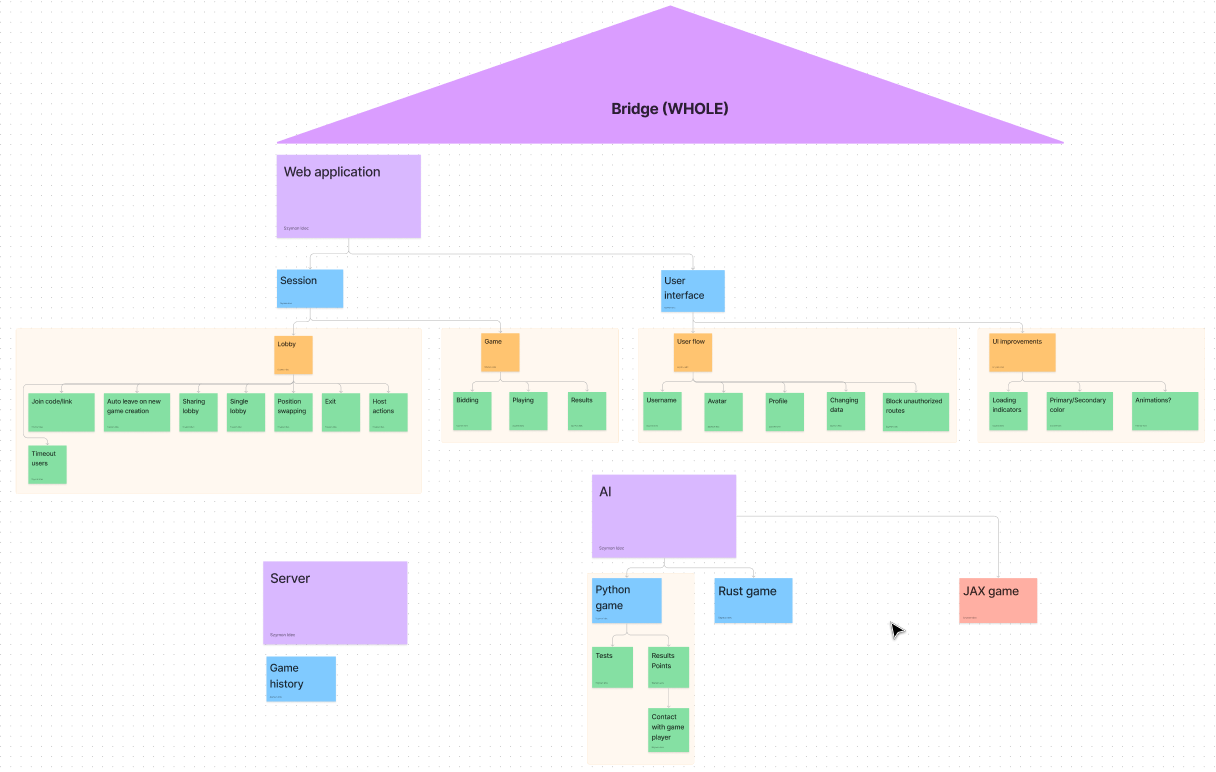
\includegraphics[width=0.9\textwidth]{img/schematy/milestones.png}
    \caption{Szczegółowy podział milestone'ów na zadania}
    \label{fig:figma_strategicplan}
\end{figure}

Opierając się na powyższym planie, można stwierdzić, że udało się
zrealizować wszystkie wymagania sprecyzowane przez klienta.
Jedynym elementem, który został zrealizowany alternatywnie,
zgodnie z~założeniami zagrożeń implementacji
(\nameref{sec:analiza_zagrozen}), był wirtualny asystent. Szczegóły
dotyczące tej części projektu zostały opisane w~sekcji dotyczącej
asystenta \nameref{subsubsec:mocai}.

\section{Przegląd zrealizowanych funkcjonalności}

\subsection{Interfejs aplikacji}

\subsubsection{Tworzenie i dołączenie do gry}
\subsubsection{Lobby}
\subsubsection{Host}
\subsubsection{Użytkownik}


\subsection{Gra w brydża}

\subsubsection{Licytacja}
\subsubsection{Rozgrywka}


\subsection{Wirtualny asystent}
%%% przeprowadzone testy aplikacji na wybranej grupie osób (do wywalenia?)

\subsubsection{Moc AI}
\label{subsubsec:mocai}
%%% testy/badania czy AI wygrywa

\subsubsection{Możliwości rozwoju modelu}
%%% czy da sie rozszerzac o kolejne elementy gry brydza
%%% mozna sie odwolac do dalszych perspektyw (na ten moment w PR)

\subsection{Ułatwienia dostępności}

\subsubsection{Intuicyjność interfejsu}
% intuicyjne ikony stosowane obszernie w sieci

\subsubsection{Responsywny układ aplikacji}
\subsubsection{Motywy jasny i ciemny}


\section{Dalsze perspektywy rozwoju projektu}

\section{Podsumowanie}


